\documentclass[tikz]{standalone}
\usepackage{pgfplots}
\pgfplotsset{compat=newest}
\pgfplotsset{every axis legend/.append style={%
cells={anchor=west}}
}
\usetikzlibrary{arrows}
\tikzset{>=stealth'}

\begin{document}
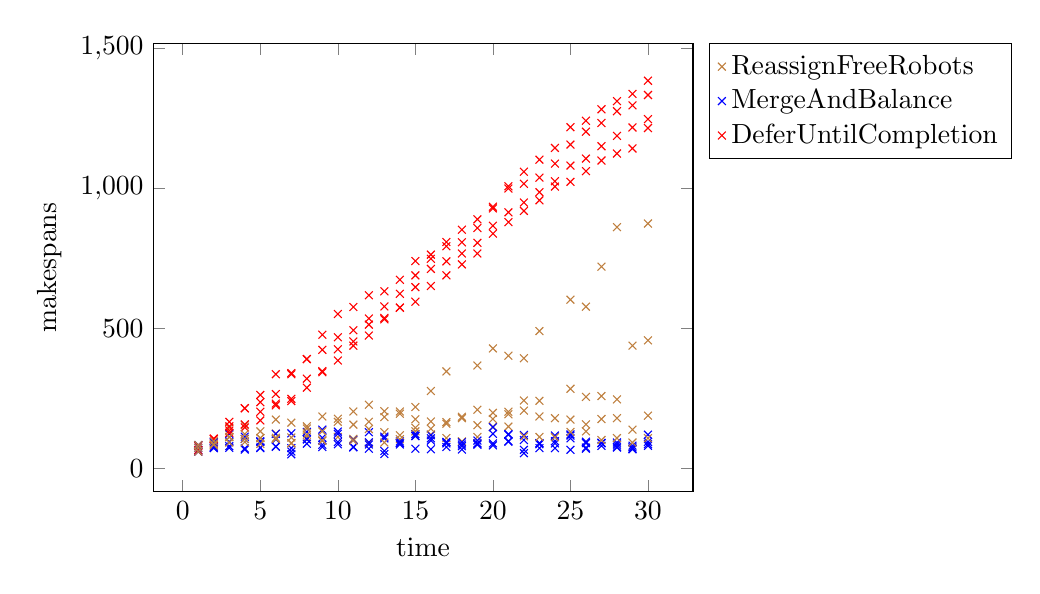
\begin{tikzpicture}[]
\begin{axis}[legend pos = {outer north east}, ylabel = {makespans}, ymode = {linear}, xlabel = {time}]\addplot+ [mark = {x}, only marks = {true}, brown,solid, mark options={solid,fill=brown}]coordinates {
(1, 66)
(2, 82)
(3, 146)
(4, 155)
(5, 109)
(6, 125)
(7, 164)
(8, 112)
(9, 101)
(10, 113)
(11, 106)
(12, 91)
(13, 130)
(14, 105)
(15, 133)
(16, 122)
(17, 109)
(18, 97)
(19, 113)
(20, 149)
(21, 150)
(22, 243)
(23, 242)
(25, 285)
(26, 256)
(27, 259)
(28, 247)
(29, 439)
(30, 458)
};
\addlegendentry{ReassignFreeRobots}
\addplot+ [mark = {x}, only marks = {true}, blue,solid, mark options={solid,fill=blue}]coordinates {
(1, 66)
(2, 78)
(3, 124)
(4, 106)
(5, 73)
(6, 79)
(7, 126)
(8, 105)
(9, 85)
(10, 95)
(11, 76)
(12, 71)
(13, 114)
(14, 97)
(15, 116)
(16, 108)
(17, 95)
(18, 68)
(19, 100)
(20, 124)
(21, 121)
(22, 102)
(23, 90)
(24, 90)
(25, 122)
(26, 71)
(27, 92)
(28, 78)
(29, 76)
(30, 95)
};
\addlegendentry{MergeAndBalance}
\addplot+ [mark = {x}, only marks = {true}, red,solid, mark options={solid,fill=red}]coordinates {
(1, 66)
(2, 93)
(3, 167)
(4, 216)
(5, 237)
(6, 266)
(7, 341)
(8, 391)
(9, 424)
(10, 469)
(11, 494)
(12, 514)
(13, 579)
(14, 624)
(15, 690)
(16, 749)
(17, 794)
(18, 808)
(19, 859)
(20, 935)
(21, 1008)
(22, 1060)
(23, 1103)
(24, 1145)
(25, 1219)
(26, 1242)
(27, 1283)
(28, 1312)
(29, 1338)
(30, 1385)
};
\addlegendentry{DeferUntilCompletion}
\addplot+ [mark = {x}, only marks = {true}, red,solid, mark options={solid,fill=red}]coordinates {
(1, 61)
(2, 105)
(3, 136)
(4, 158)
(5, 203)
(6, 232)
(7, 241)
(8, 321)
(9, 344)
(10, 426)
(11, 454)
(12, 536)
(13, 538)
(14, 575)
(15, 648)
(16, 713)
(17, 740)
(18, 768)
(19, 806)
(20, 839)
(21, 880)
(22, 950)
(23, 987)
(24, 1007)
(25, 1024)
(26, 1062)
(27, 1100)
(28, 1125)
(29, 1143)
(30, 1216)
};
\addplot+ [mark = {x}, only marks = {true}, red,solid, mark options={solid,fill=red}]coordinates {
(1, 80)
(2, 107)
(3, 151)
(4, 215)
(5, 263)
(6, 337)
(7, 337)
(8, 391)
(9, 478)
(10, 552)
(11, 577)
(12, 619)
(13, 633)
(14, 674)
(15, 741)
(16, 764)
(17, 809)
(18, 853)
(19, 890)
(20, 929)
(21, 1000)
(22, 1017)
(23, 1039)
(24, 1089)
(25, 1157)
(26, 1203)
(27, 1234)
(28, 1276)
(29, 1297)
(30, 1334)
};
\addplot+ [mark = {x}, only marks = {true}, red,solid, mark options={solid,fill=red}]coordinates {
(1, 84)
(2, 107)
(3, 128)
(4, 147)
(5, 172)
(6, 226)
(7, 249)
(8, 289)
(9, 348)
(10, 386)
(11, 439)
(12, 475)
(13, 533)
(14, 574)
(15, 596)
(16, 652)
(17, 690)
(18, 729)
(19, 768)
(20, 867)
(21, 915)
(22, 920)
(23, 958)
(24, 1026)
(25, 1082)
(26, 1107)
(27, 1151)
(28, 1188)
(29, 1218)
(30, 1248)
};
\addplot+ [mark = {x}, only marks = {true}, blue,solid, mark options={solid,fill=blue}]coordinates {
(1, 61)
(2, 94)
(3, 80)
(4, 72)
(5, 95)
(6, 78)
(7, 61)
(8, 131)
(9, 77)
(10, 132)
(11, 78)
(12, 130)
(13, 52)
(14, 86)
(15, 123)
(16, 119)
(17, 77)
(18, 80)
(19, 90)
(20, 83)
(21, 96)
(22, 120)
(23, 91)
(24, 73)
(25, 67)
(26, 91)
(27, 90)
(28, 75)
(29, 69)
(30, 121)
};
\addplot+ [mark = {x}, only marks = {true}, blue,solid, mark options={solid,fill=blue}]coordinates {
(1, 74)
(2, 74)
(3, 96)
(4, 114)
(5, 98)
(6, 124)
(7, 51)
(8, 104)
(9, 139)
(10, 124)
(11, 76)
(12, 94)
(13, 63)
(14, 91)
(15, 117)
(16, 69)
(17, 95)
(18, 94)
(19, 85)
(20, 90)
(21, 123)
(22, 67)
(23, 73)
(24, 98)
(25, 118)
(26, 96)
(27, 81)
(28, 93)
(29, 71)
(30, 87)
};
\addplot+ [mark = {x}, only marks = {true}, blue,solid, mark options={solid,fill=blue}]coordinates {
(1, 84)
(2, 73)
(3, 74)
(4, 68)
(5, 75)
(6, 104)
(7, 73)
(8, 89)
(9, 110)
(10, 87)
(11, 102)
(12, 86)
(13, 108)
(14, 91)
(15, 71)
(16, 100)
(17, 90)
(18, 86)
(19, 89)
(20, 148)
(21, 98)
(22, 55)
(23, 87)
(24, 118)
(25, 108)
(26, 75)
(27, 92)
(28, 86)
(29, 82)
(30, 81)
};
\addplot+ [mark = {x}, only marks = {true}, brown,solid, mark options={solid,fill=brown}]coordinates {
(1, 61)
(2, 98)
(3, 113)
(4, 95)
(5, 109)
(6, 110)
(7, 90)
(8, 151)
(9, 99)
(10, 178)
(11, 100)
(12, 141)
(13, 93)
(14, 119)
(15, 146)
(16, 168)
(17, 166)
(18, 180)
(19, 210)
(20, 199)
(21, 203)
(22, 207)
(23, 186)
(24, 180)
(25, 175)
(26, 158)
(27, 177)
(28, 180)
(29, 139)
(30, 189)
};
\addplot+ [mark = {x}, only marks = {true}, brown,solid, mark options={solid,fill=brown}]coordinates {
(1, 74)
(2, 85)
(3, 112)
(4, 123)
(5, 133)
(6, 175)
(7, 111)
(8, 143)
(9, 186)
(11, 204)
(12, 228)
(13, 184)
(14, 204)
(15, 220)
(16, 142)
(17, 160)
(18, 185)
(19, 155)
(20, 177)
(21, 194)
(22, 115)
(23, 113)
(24, 112)
(25, 131)
(26, 133)
(27, 102)
(28, 109)
(29, 93)
(30, 109)
};
\addplot+ [mark = {x}, only marks = {true}, brown,solid, mark options={solid,fill=brown}]coordinates {
(1, 84)
(2, 88)
(3, 93)
(4, 106)
(5, 88)
(6, 106)
(7, 91)
(8, 121)
(9, 133)
(10, 167)
(11, 157)
(12, 167)
(13, 205)
(14, 196)
(15, 176)
(16, 277)
(17, 347)
(19, 368)
(20, 429)
(21, 403)
(22, 394)
(23, 491)
(25, 603)
(26, 578)
(27, 721)
(28, 862)
(30, 875)
};
\end{axis}

\end{tikzpicture}
\end{document}
